

This element pair is discussed in 5.3.3 of Elman, Silvester and Wathen: 

``[Another] possibility is to construct a hybrid pressure approximation by 
combining the continuous linear pressure approximation with the discontinuous constant pres-
sure approximation. The resulting mixed method is referred to as the $P_2-P_{-1*}$ 
approximation and enjoys the best of both worlds; it has locally 
incompressibility, and yet it does not have its accuracy compromised by
the lower order pressure [of $P_2\times P_0$]. 
Perhaps surprisingly, this element is also uniformly stable.'' 

\begin{center}
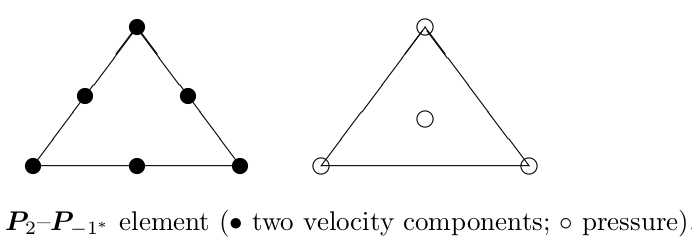
\includegraphics[width=7cm]{images/pair_p2p1p0/elsw}\\
{\captionfont Taken from \textcite{elsw}.}
\end{center}

In Gresho \& Sani table 3.13-1: ``LBB stable yes. Better than P2P1, element mass balance.
more work than P2P1. 2 hydrostatic modes. Second order.'' 
Note that they call it P2(P1+P0) and that they call the CR element P2+P1 (not P-1) so that 
I don't know whether its pressure is continuous or not. However since they state 'element mass balance'
it probably means disc pressure. On the other hand, the drawing and legend of this element in the table 
is clear: pressure at the 3 vertices is continuous and there is a cross (disc pressure) in the middle. 

\begin{center}
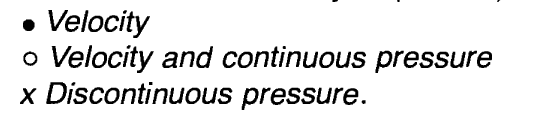
\includegraphics[width=4cm]{images/pair_p2p1p0/grsa2}
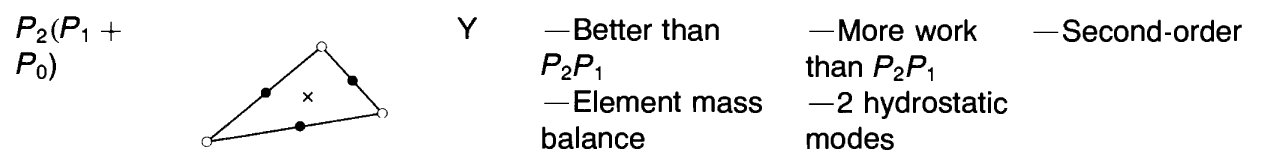
\includegraphics[width=12cm]{images/pair_p2p1p0/grsa1}\\
{\captionfont Taken from \textcite{grsa}.}
\end{center}

\textcite{bocg12} (2012) state: ``[...] the pressure space $Q_h$ is defined as the sum of two finite 
element spaces, namely $P_k+P_0$ ($k \ge d- 1$) [...]for the enhanced Hood–Taylor [...]. 
However, it can be easily observed that the sum is not direct, 
since globally constant functions can be represented exactly by means of piecewise 
$P_0$ or continuous $P_k$ ($k \ge 1$) elements.
Concerning the implementation of the method, we avoid the computation of the basis
functions of such a finite element by testing the discrete problem (2.3) with the basis 
functions of the two subspaces separately. By the above discussion it turns out that the resulting
matrix is rank-deficient, with kernel of dimension 1.''


